% This is text associated with the open textbook "Open Electromagnetics"
% See immediately below for author, date
% <License info goes here (boilerplate, not read by project compiler)>

%ORB TITLE Potential Induced in a Dipole
%ORB AUTHOR 0        # S.W. Ellingson, Virginia Tech (ellingson@vt.edu)
%ORB DATE 20191212   # yyyymmdd
%ORB ABSTRACT 

\label{m0215_Voltage_Induced_in_a_Dipole} % <-- Must match name of this file and module directory name.  Don't mess with this!

An electromagnetic wave incident on an antenna will induce a potential at the terminals of the antenna.
In this section, we shall derive this potential.
To simplify the derivation, we shall consider the special case of a straight thin dipole of arbitrary length that is illuminated by a plane wave.
However, certain aspects of the derivation will apply to antennas generally.
In particular, the concepts of \emph{effective length}
\index{effective length}
(also known as \emph{effective height}) and
\emph{vector effective length} 
\index{vector effective length}
emerge naturally from this derivation, so this section also serves as a stepping stone in the development of an equivalent circuit model for a receiving antenna.
The derivation relies on the transmit properties of dipoles as well as the principle of reciprocity, 
so familiarity with those topics is recommended before reading this section.

The scenario of interest is shown in Figure~\ref{m0215_fRxDipole}.
Here a thin $\hat{\bf z}$-aligned straight dipole is located at the origin.
The total length of the dipole is $L$. 
The arms of the dipole are perfectly-conducting.
The terminals consist of a small gap of length $\Delta l$ between the arms. 
The incident plane wave is described in terms of its electric field intensity $\widetilde{\bf E}^i$.
The question is: What is $\widetilde{V}_{OC}$, the potential at the terminals when the terminals are open-circuited?
%
\begin{figure}[b!] % <--- "[b!]" for first figure in section *only*; delete for 2nd and subsequent figures
\begin{center}
\pdftooltip{{  % note double braces
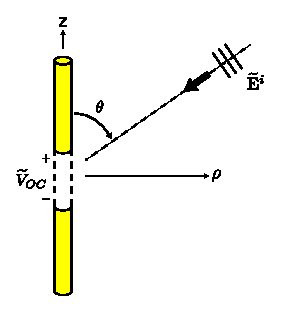
\includegraphics[width=2in]{modules/m0215_fRxDipole.eps} 
% https://commons.wikimedia.org/wiki/File:Thin_straight_dipole_respond_to_incident_plane_wave.svg
}}{A rho-z coordinate system with a wire along the z axis. The wire has a cutout labeled capital V tilde sub quantity capital o capital c. A dashed line is an angle theta from the positive z axis. Along the dashed line is a plane wave labeled capital e tilde superscript small i pointing toward the origin.}
\end{center}
\centerline{\scriptsize 
\copyright~\hyperref[m0215_fRxDipole_Credit]{C.\ Wang} 
\href{https://creativecommons.org/licenses/by-sa/4.0/}{CC BY-SA 4.0} 
} % \centerline 
\caption{
\label{m0215_fRxDipole}
A potential is induced at the terminals of a thin straight dipole in response to an incident plane wave.
}
\end{figure}

There are multiple approaches to solve this problem.
A direct attack is to invoke the principle that potential is equal to the integral of the electric field intensity over a path.
In this case, the path begins at the ``$-$'' terminal and ends at the ``$+$'' terminal, crossing the gap that defines the antenna terminals.
Thus:
%
\begin{equation}
\widetilde{V}_{OC} = -\int_{gap} \widetilde{\bf E}_{gap} \cdot d{\bf l}
\label{m0215_eVoc-General}
\end{equation}
%
where $\widetilde{\bf E}_{gap}$ is the electric field in the gap.
The problem with this approach is that the value of $\widetilde{\bf E}_{gap}$ is not readily available.
It is not simply $\widetilde{\bf E}^i$, because the antenna structure (in particular, the electromagnetic boundary conditions)
\index{boundary conditions}
modify the electric field in the vicinity of the antenna.\footnote{Also, if this were true, then the antenna itself would not matter; only the relative spacing and orientation of the antenna terminals would matter!}

Fortunately, we can bypass this obstacle using the principle of reciprocity.
In a reciprocity-based strategy, we establish a relationship between two scenarios that take place within the same electromagnetic system.
The first scenario is shown in Figure~\ref{m0215_fReciprocity1}.
%
\begin{figure} % <--- "[b!]" for first figure in section *only*; delete for 2nd and subsequent figures
\begin{center}
\pdftooltip{{  % note double braces
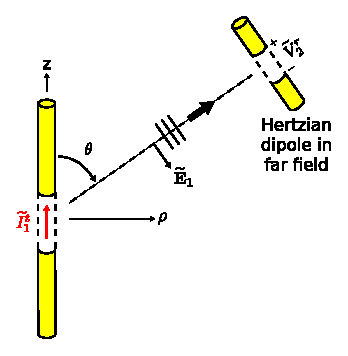
\includegraphics[width=2.5in]{modules/m0215_fReciprocity1.eps} 
% https://commons.wikimedia.org/wiki/File:Dipole_of_interest_driven_by_current.svg
}}{A rho-z coordinate system with a wire along the z axis. The wire has a cutout labeled capital I tilde subscript 1 superscript t. A dashed line is an angle theta from the positive z axis. Along the dashed line is a plane wave moving away from the origin. Capital e tilde subscript 1 is perpendicular to the dashed line (clockwise). Plane wave approaches a second dipole wire with cutout capital v tilde subscript 2 superscript r.
}
\end{center}
\centerline{\scriptsize 
\copyright~\hyperref[m0215_fReciprocity1_Credit]{C.\ Wang} 
\href{https://creativecommons.org/licenses/by-sa/4.0/}{CC BY-SA 4.0} 
} % \centerline 
\caption{
\label{m0215_fReciprocity1}
The dipole of interest driven by current $\widetilde{I}_1^t$ radiates electric field $\widetilde{\bf E}_1$, resulting in open-circuit potential $\widetilde{V}_2^r$ at the terminals of a Hertzian dipole in the far field.
}
\end{figure}
%
\begin{figure} % <--- "[b!]" for first figure in section *only*; delete for 2nd and subsequent figures
\begin{center}
\pdftooltip{{  % note double braces
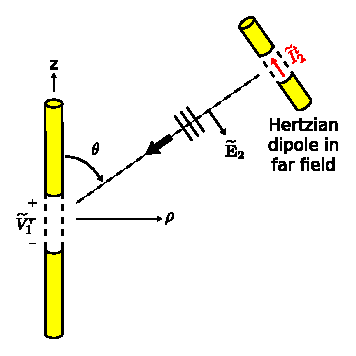
\includegraphics[width=2.5in]{modules/m0215_fReciprocity2.eps} 
% https://commons.wikimedia.org/wiki/File:Hertzian_dipole_drive_by_current.svg
}}{A rho-z coordinate system with a wire along the z axis. The wire has a cutout labeled capital V tilde subscript 1 superscript r. A dashed line is an angle theta from the positive z axis. Along the dashed line is a plane wave moving toward the origin. Capital e tilde subscript 2 is perpendicular to the dashed line (clockwise). Plane wave moves away from a second dipole wire with cutout capital I tilde subscript 2 superscript t.}
\end{center}
\centerline{\scriptsize 
\copyright~\hyperref[m0215_fReciprocity2_Credit]{C.\ Wang} 
\href{https://creativecommons.org/licenses/by-sa/4.0/}{CC BY-SA 4.0} 
} % \centerline 
\caption{
\label{m0215_fReciprocity2}
The Hertzian dipole driven by current $\widetilde{I}_2^t$ radiates electric field $\widetilde{\bf E}_2$, resulting in open-circuit potential $\widetilde{V}_1^r$ at the terminals of the dipole of interest.
}
\end{figure}
%
In this scenario, we have two dipoles.
The first dipole is precisely the dipole of interest (Figure~\ref{m0215_fRxDipole}), \emph{except} that a current $\widetilde{I}_1^t$ is applied to the antenna terminals.
This gives rise to a current distribution $\widetilde{I}(z)$ (SI base units of A) along the dipole, and subsequently the dipole radiates the electric field (Section~\ref{m0199_Radiation_from_a_Thin_Straight_Filament_of_Current}):
%
\begin{flalign}
\widetilde{\bf E}_1({\bf r}) &\approx \hat{\bf \theta} j \frac{\eta}{2} \frac{e^{-j\beta r}}{r}~\left(\sin\theta\right) \nonumber \\
                           & ~~~\cdot\left[\frac{1}{\lambda}\int_{-L/2}^{+L/2} \widetilde{I}(z') e^{+j\beta z'\cos{\theta}} dz'\right] 
\label{m0215_eESDE}
\end{flalign}
%
The second antenna is a $\hat{\bf \theta}$-aligned Hertzian dipole 
\index{Hertzian dipole}
in the far field, which receives $\widetilde{\bf E}_1$.  
(For a refresher on the properties of Hertzian dipoles, see Section~\ref{m0197_Radiation_from_a_Hertzian_Dipole}. A key point is that Hertzian dipoles are vanishingly small.)
Specifically, we measure (conceptually, at least) the open-circuit potential $\widetilde{V}_2^r$ at the terminals of the Hertzian dipole.
We select a Hertzian dipole for this purpose because -- in contrast to essentially all other antennas -- it is simple to determine the open circuit potential.  As explained earlier:
%
\begin{equation}
\widetilde{V}_2^r = -\int_{gap} \widetilde{\bf E}_{gap} \cdot d{\bf l}
\end{equation}
%
For the Hertzian dipole, $\widetilde{\bf E}_{gap}$ \emph{is} simply the incident electric field, since there is negligible structure (in particular, a negligible amount of material) present to modify the electric field.
Thus, we have simply:
%
\begin{equation}
\widetilde{V}_2^r = -\int_{gap} \widetilde{\bf E}_1 \cdot d{\bf l}
\label{m0215_eV2r1}
\end{equation}
%
Since the Hertzian dipole is very short and very far away from the transmitting dipole, $\widetilde{\bf E}_1$ is essentially constant over the gap.  Also recall that we required the Hertzian dipole to be aligned with $\widetilde{\bf E}_1$.
Choosing to integrate in a straight line across the gap, Equation~\ref{m0215_eV2r1} reduces to:
%
\begin{equation}
\widetilde{V}_2^r = -\widetilde{\bf E}_1({\bf r}_2) \cdot \hat{\bf \theta}\Delta l
\label{m0215_eV2r2}
\end{equation}
%
where $\Delta l$ is the length of the gap and ${\bf r}_2$ is the location of the Hertzian dipole.
Substituting the expression for $\widetilde{\bf E}_1$ from Equation~\ref{m0215_eESDE}, we obtain:
%
\begin{flalign}
\widetilde{V}_2^r \approx &- j \frac{\eta}{2} \frac{e^{-j\beta r_2}}{r_2}~\left(\sin\theta\right) \nonumber \\
                           & ~~~\cdot\left[\frac{1}{\lambda}\int_{-L/2}^{+L/2} \widetilde{I}(z') e^{+j\beta z'\cos{\theta}} dz'\right] \Delta l
\label{m0215_eV2r3}
\end{flalign}
%
where $r_2=\left|{\bf r}_2\right|$. 

The second scenario is shown in Figure~\ref{m0215_fReciprocity2}.
%
This scenario is identical to the first scenario, with the exception that the Hertzian dipole transmits and the dipole of interest receives.
The field radiated by the Hertzian dipole in response to applied current $\widetilde{I}_2^t$, evaluated at the origin, is (Section~\ref{m0197_Radiation_from_a_Hertzian_Dipole}):
%
\begin{equation}
\widetilde{\bf E}_2({\bf r}=0) \approx \hat{\bf \theta} j\eta \frac{\widetilde{I}_2^t\cdot\beta \Delta l}{4\pi}~(1)~\frac{e^{-j\beta r_2}}{r_2} 
\label{m0215_eE}
\end{equation}
%
The ``$\sin\theta$'' factor in the general expression is equal to 1 in this case, since, as shown in Figure~\ref{m0215_fReciprocity2}, the origin is located broadside (i.e., at $\pi/2$~rad) relative to the axis of the Hertzian dipole.
Also note that because the Hertzian dipole is presumed to be in the far field, ${\bf E}_2$ may be interpreted as a plane wave in the region of the receiving dipole of interest.

Now we ask: What is the induced potential $\widetilde{V}_1^r$ in the dipole of interest?
Once again, Equation~\ref{m0215_eVoc-General} is not much help, because the electric field in the gap is not known.
However, we do know that $\widetilde{V}_1^r$ should be proportional to $\widetilde{\bf E}_2({\bf r}=0)$, since this is presumed to be a linear system.
Based on this much information alone, there must be some vector ${\bf l}_e=\hat{\bf l} l_e$ for which
%
\begin{equation}
\widetilde{V}_1^r = \widetilde{\bf E}_2({\bf r}=0) \cdot {\bf l}_e
\label{m0215_eVEL1}
\end{equation}
%
This does not uniquely define either the unit vector $\hat{\bf l}$ nor the scalar part $l_e$, since a change in the definition of the former can be compensated by a change in the definition of the latter and vice-versa.
So at this point we invoke the standard definition of ${\bf l}_e$ as the \emph{vector effective length},
\index{vector effective length}
introduced in Section~\ref{m0206_Equivalent_Circuit_Model_for_Reception}.
Thus, $\hat{\bf l}$ is defined to be the direction in which an electric field \emph{transmitted} from the antenna would be polarized.
In the present example, $\hat{\bf l}=-\hat{\bf \theta}$, where the minus sign reflects the fact that positive terminal potential results in terminal current which flows in the $-\hat{\bf z}$ direction. 
Thus, Equation~\ref{m0215_eVEL1} becomes:
%
\begin{equation}
\widetilde{V}_1^r = -\widetilde{\bf E}_2({\bf r}=0) \cdot \hat{\bf \theta} l_e
\end{equation}
%
We may go a bit further and substitute the expression for $\widetilde{\bf E}_2({\bf r}=0)$ from Equation~\ref{m0215_eE}:
%
\begin{equation}
\widetilde{V}_1^r \approx - j\eta~\frac{\widetilde{I}_2^t\cdot\beta \Delta l}{4\pi}~\frac{e^{-j\beta r_2}}{r_2} l_e
\label{m0215_eV1r1}
\end{equation}

Now we invoke reciprocity.  As a two-port linear time-invariant system, it must be true that:
%
\begin{equation}
\widetilde{I}_1^t \widetilde{V}_1^r = \widetilde{I}_2^t \widetilde{V}_2^r
\end{equation}
%
Thus:
%
\begin{equation}
\widetilde{V}_1^r = \frac{\widetilde{I}_2^t}{\widetilde{I}_1^t} \widetilde{V}_2^r
\end{equation}
%
Substituting the expression for $\widetilde{V}_2^r$ from Equation~\ref{m0215_eV2r3}:
%
\begin{flalign}
\widetilde{V}_1^r \approx &- \frac{\widetilde{I}_2^t}{\widetilde{I}_1^t} \cdot j \frac{\eta}{2} \frac{e^{-j\beta r_2}}{r_2}~\left(\sin\theta\right) \nonumber \\
                           & ~~~\cdot\left[\frac{1}{\lambda}\int_{-L/2}^{+L/2} \widetilde{I}(z') e^{+j\beta z'\cos{\theta}} dz'\right] \Delta l
\end{flalign}
%
Thus, reciprocity has provided a second expression for $\widetilde{V}_1^r$.
We may solve for $l_e$ by setting this expression equal to the expression from Equation~\ref{m0215_eV1r1}, yielding
%
\begin{equation}
l_e \approx \frac{2\pi}{\beta \widetilde{I}_1^t} \left[\frac{1}{\lambda}\int_{-L/2}^{+L/2} \widetilde{I}(z') e^{+j\beta z'\cos{\theta}} dz'\right] \sin\theta
\end{equation}
%
Noting that $\beta=2\pi/\lambda$, this simplifies to:
%
\begin{equation}
l_e \approx \left[ \frac{1}{\widetilde{I}_1^t}\int_{-L/2}^{+L/2} \widetilde{I}(z') e^{+j\beta z'\cos{\theta}} dz' \right] \sin\theta
\label{m0215_ele}
\end{equation}
%
Thus, you can calculate $l_e$ using the following procedure:
%
\begin{enumerate}
\item Apply a current $\widetilde{I}_1^t$ to the dipole of interest.
\item Determine the resulting current distribution $\widetilde{I}(z)$ along the length of the dipole.  (Note that precisely this is done for the electrically-short dipole in Section~\ref{m0198_Radiation_from_an_Electrically-Short_Dipole} and for the half-wave dipole in Section~\ref{m0200_Radiation_from_a_Half-Wave_Dipole}.)
\item Integrate $\widetilde{I}(z)$ over the length of the dipole as indicated in Equation~\ref{m0215_ele}. Then divide (``normalize'') by $\widetilde{I}_1^t$ (which is simply $\widetilde{I}(0)$).  Note that the result is independent of the excitation $\widetilde{I}_1^t$, as expected since this is a linear system.
\item Multiply by $\sin\theta$.
\end{enumerate}

We have now determined that the open-circuit terminal potential $\widetilde{V}_{OC}$ in response to an incident electric field $\widetilde{\bf E}^i$ is
%
\begin{equation}
\boxed{
\widetilde{V}_{OC} = \widetilde{\bf E}^i \cdot {\bf l}_e
}
\label{m0215_eVOCEL}
\end{equation}
%
where ${\bf l}_e = \hat{\bf l} l_e$ is the vector effective length defined previously.

This result is remarkable. In plain English, we have found that: 
%
%%%%%%%%%%%%%%%%%%%%%%%%%%%%%%%%%%%%%%%%%%%%%%%
%ORB HIGHLIGHT
\begin{mdframed}[backgroundcolor=yellow!20,nobreak=true] 
The potential induced in a dipole is the co-polarized component of the incident electric field times a normalized integral of the \emph{transmit} current distribution over the length of the dipole, times sine of the angle between the dipole axis and the direction of incidence. 
%(Equation~\ref{m0215_ele}).
\end{mdframed}
%%%%%%%%%%%%%%%%%%%%%%%%%%%%%%%%%%%%%%%%%%%%%%%
%
In other words, the reciprocity property of linear systems allows this property of a receiving antenna to be determined relatively easily if the transmit characteristics of the antenna are known. 

%%%%%%%%%%%%%%%%%%%%%%%%%%%%%%%%%%%%%%%%%%%%%%%
%ORB EXAMPLE
~\\ \begin{example} 
\label{m0215_exESD}
\begin{mdframed}[backgroundcolor=brown!20,linecolor=brown!20]\raggedright
Effective length of a thin electrically-short dipole (ESD).
\\~\\
A explained in Section~\ref{m0198_Radiation_from_an_Electrically-Short_Dipole}, the current distribution on a thin ESD is
%
\begin{equation}
\widetilde{I}(z) \approx I_0 \left(1-\frac{2}{L}\left|z\right|\right) 
\end{equation}
%
where $L$ is the length of the dipole and $I_0$ is the terminal current.
Applying Equation~\ref{m0215_ele}, we find:
%
\begin{flalign}
l_e \approx & \left[ \frac{1}{I_0}\int_{-L/2}^{+L/2} I_0 \left(1-\frac{2}{L}\left|z'\right|\right) e^{+j\beta z'\cos{\theta}} dz' \right] \nonumber \\ 
            &\cdot \sin\theta
\end{flalign}
%
Recall $\beta=2\pi/\lambda$, so $\beta z'=2\pi\left(z'/\lambda\right)$. 
Since this is an \emph{electrically-short} dipole, $z' \ll \lambda$ over the entire integral, and subsequently we may assume $e^{+j\beta z'\cos{\theta}}\approx 1$ over the entire integral. Thus:
%
\begin{equation}
l_e \approx \left[ \int_{-L/2}^{+L/2} \left(1-\frac{2}{L}\left|z'\right|\right) dz' \right] \sin\theta
\end{equation}
%
The integral is easily solved using standard methods, or simply recognize that the ``area under the curve'' in this case is simply one-half ``base'' ($L$) times ``height'' ($1$).  Either way, we find 
%
\begin{equation}
l_e\approx \frac{L}{2} \sin\theta
\end{equation}

\end{mdframed}
% note figures will need to go between "\end{mdframed}" and "\end{example}"
\end{example}
%%%%%%%%%%%%%%%%%%%%%%%%%%%%%%%%%%%%%%%%%%%%%%%

Example~\ref{m0206_exIPESD} (Section~\ref{m0206_Equivalent_Circuit_Model_for_Reception}) demonstrates how Equation~\ref{m0215_eVOCEL} with the vector effective length determined in the preceding example is used to obtain the induced potential.

